% Created 2016-04-26 Tue 09:59
\documentclass[10pt,t,a4paper]{article}
\usepackage[utf8]{inputenc}
\usepackage[T1]{fontenc}
\usepackage{fixltx2e}
\usepackage{graphicx}
\usepackage{grffile}
\usepackage{longtable}
\usepackage{wrapfig}
\usepackage{rotating}
\usepackage[normalem]{ulem}
\usepackage{amsmath}
\usepackage{textcomp}
\usepackage{amssymb}
\usepackage{capt-of}
\usepackage{hyperref}
\author{Mikael Svahnberg\thanks{Mikael.Svahnberg@bth.se}}
\date{2016-04-21}
\title{Mapping Design to Code}
\hypersetup{
 pdfauthor={Mikael Svahnberg},
 pdftitle={Mapping Design to Code},
 pdfkeywords={},
 pdfsubject={},
 pdfcreator={Emacs 25.1.50.1 (Org mode 8.3.4)}, 
 pdflang={English}}
\begin{document}

\maketitle

\section{Warmup}
\label{sec:orgheadline5}
\subsection{Example: From Class Diagram to Code\hfill{}\textsc{Example}}
\label{sec:orgheadline1}
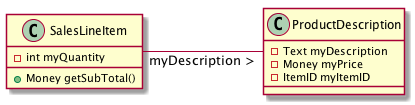
\includegraphics[width=.9\linewidth]{FClassToCode.png}

\begin{verbatim}
public class SalesLineItem {
private int myQuantity;
private ProductDescription myDescription;

public SalesLineItem(ProductDescription theDescription, int theQuantity) {...};

public Money getSubTotal() {...};
}
\end{verbatim}

\subsection{Example: From Interaction Diagrams to Code\hfill{}\textsc{Example}}
\label{sec:orgheadline2}
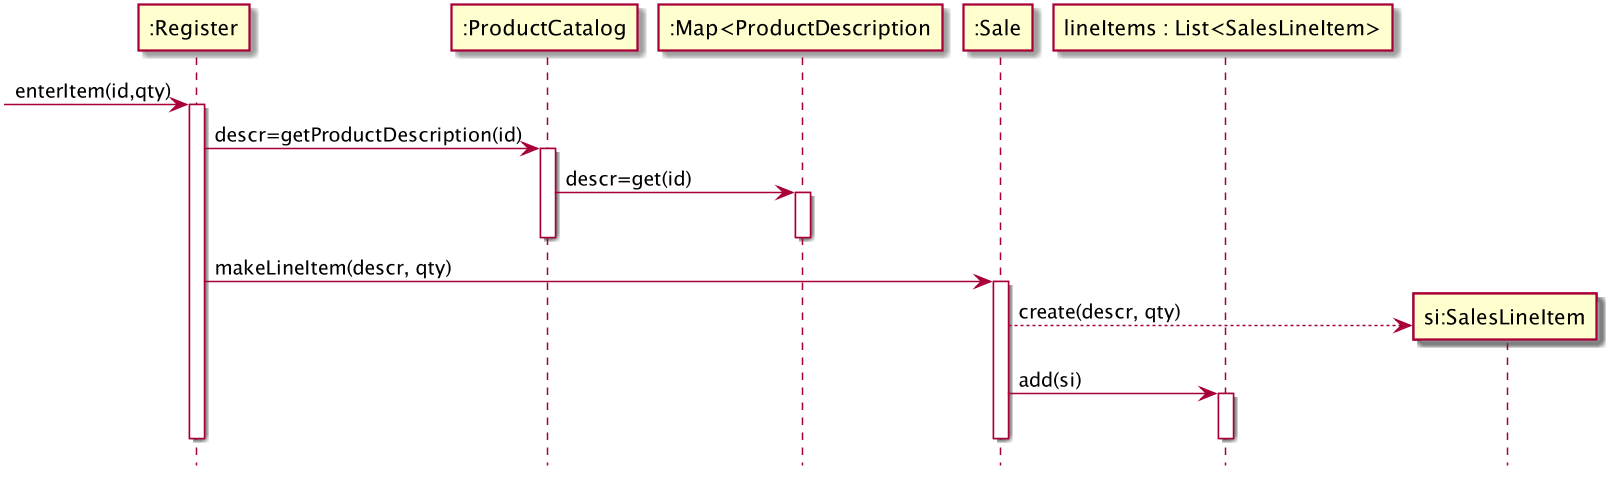
\includegraphics[width=.9\linewidth]{FInteractionToCode.png}

\subsection{Example: Collections\hfill{}\textsc{Example}}
\label{sec:orgheadline3}
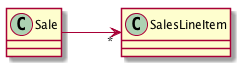
\includegraphics[width=.9\linewidth]{FCollectionsToCode.png}

\begin{verbatim}
public class Sale {
  private List<SalesLineItem> myItems = new ArrayList<SalesLineItem>;
}
\end{verbatim}

\begin{verbatim}
class Sale {
private:
  std::list<SalesLineItem*> myItems;
}
\end{verbatim}
\subsection{Discuss: Order of Implementation\hfill{}\textsc{Discussion}}
\label{sec:orgheadline4}
\begin{itemize}
\item In which order should classes be implemented?
\begin{itemize}
\item Larman: ``Least coupled to most coupled''
\item Other suggestions:
\begin{itemize}
\item Use case per use case, create stubs first, fill them out as you go.
\item First write test cases per use case, then add methods to classes (and create classes) to pass the tests.
\item First write interfaces for all classes, then inherit and implement the classes
\end{itemize}
\end{itemize}
\end{itemize}
\section{Dictionary Example}
\label{sec:orgheadline15}
\subsection{Task}
\label{sec:orgheadline7}
\begin{enumerate}
\item Dictionary
\label{sec:orgheadline6}
Write a dictionary program where you have words and their definitions.
\begin{itemize}
\item Users shall be able to browse all words.
\item Users shall be able to search for words
\item Users shall be able to search for definitions.
\item The system shall maintain a log of activities.
\item Other requirements:
\begin{itemize}
\item The system shall use a graphical user interface
\item The system shall store the words and their definitions between sessions.
\end{itemize}
\end{itemize}
\end{enumerate}
\subsection{Conceptual Model}
\label{sec:orgheadline8}
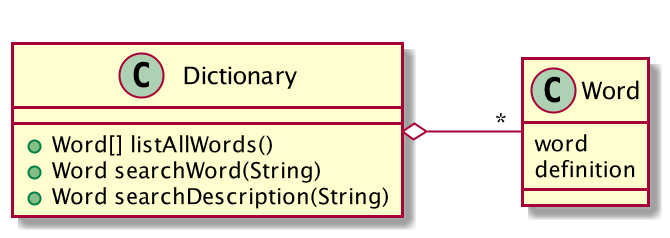
\includegraphics[width=.9\linewidth]{FDictionaryConceptual.png}

\subsection{Class Diagram I}
\label{sec:orgheadline9}
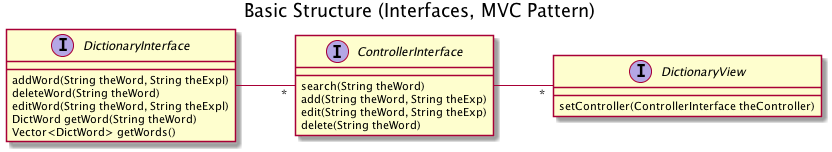
\includegraphics[width=.9\linewidth]{FDictionaryClass1.png}

\subsection{Class Diagram II}
\label{sec:orgheadline10}
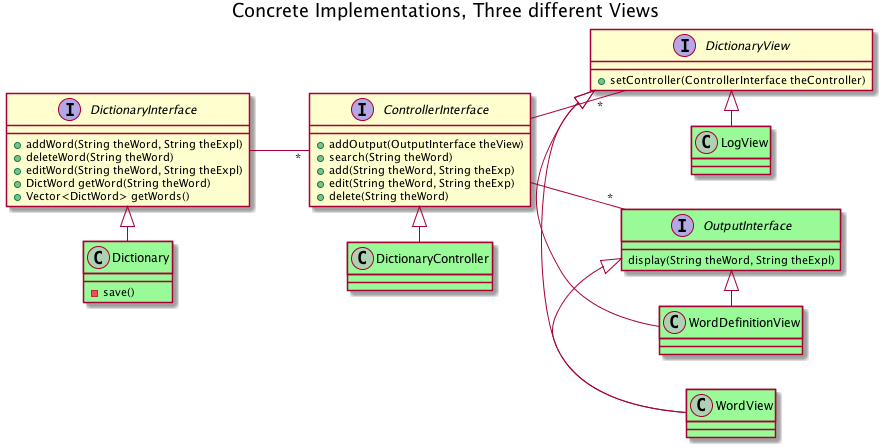
\includegraphics[width=.9\linewidth]{FDictionaryClass2.png}

\subsection{Class Diagram III}
\label{sec:orgheadline11}
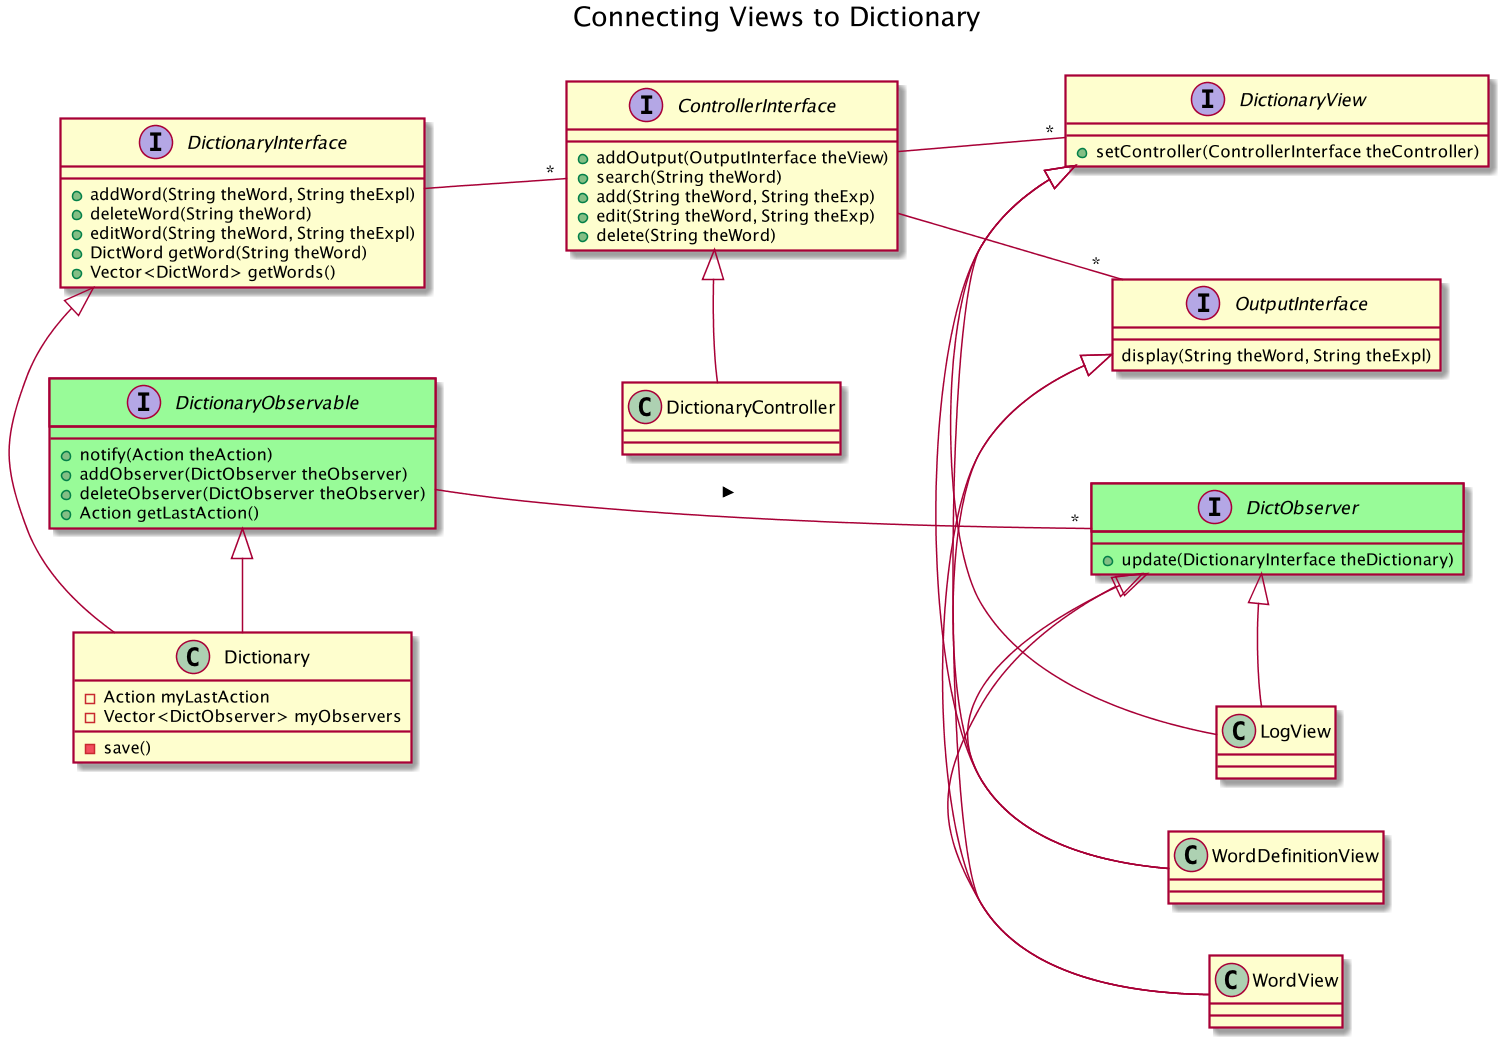
\includegraphics[width=.9\linewidth]{FDictionaryClass3.png}

\subsection{Class Diagram IV}
\label{sec:orgheadline12}
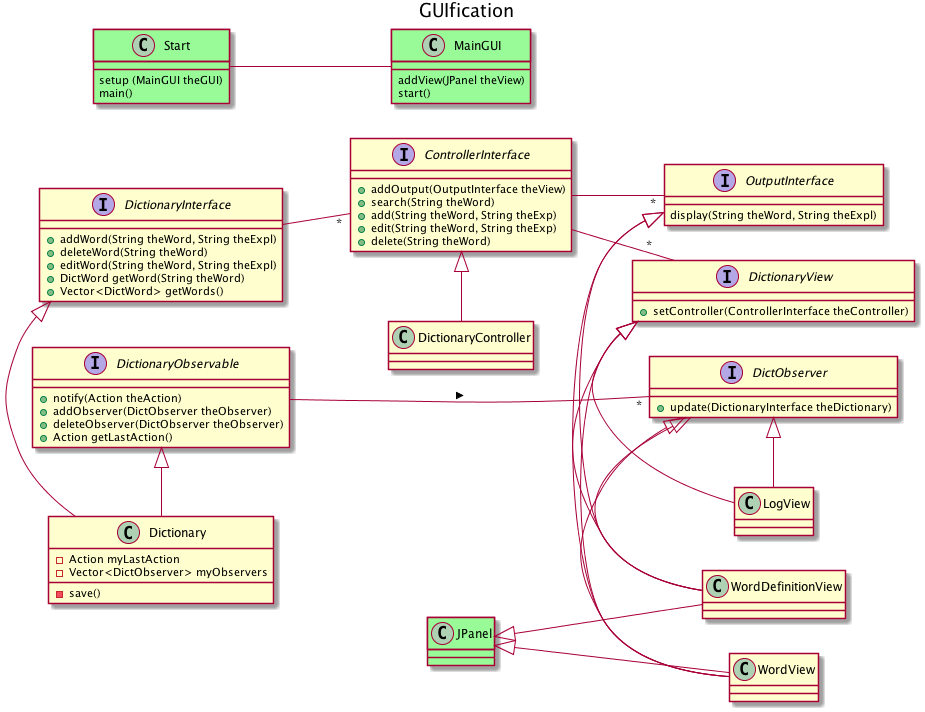
\includegraphics[width=.9\linewidth]{FDictionaryClass4.png}

\subsection{Class Diagram: setup method}
\label{sec:orgheadline13}
\begin{verbatim}
public static void setup(MainGUI theGUI) {
  // Create Dictionary
  Dictionary theDict = new Dictionary("dict.txt");
  debugDict(theDict); // Make sure there is stuff in it.

  // Create Views
  LogView lv=new LogView();
  WordView wv=new WordView();
  WordDefinitionView wdv=new WordDefinitionView();

  // Initialise views where necessary
  wv.getWords(theDict);

  // Create and Connect the Controller
  DictionaryController dc=new DictionaryController(theDict, wdv);
  lv.setController(dc);
  wv.setController(dc);
  wdv.setController(dc); // Circular, but ok

  // Add stuff to GUI
  // theGUI.addView(lv) // skip the LogView; it prints to console/file
  theGUI.addView(wv);
  theGUI.addView(wdv);

  // Connect views to dictionary, so that changes are reflected
  theDict.addObserver(lv);
  theDict.addObserver(wv);
  theDict.addObserver(wdv);
}
\end{verbatim}
\subsection{Discussion: Order of Implementation\hfill{}\textsc{Discussion}}
\label{sec:orgheadline14}
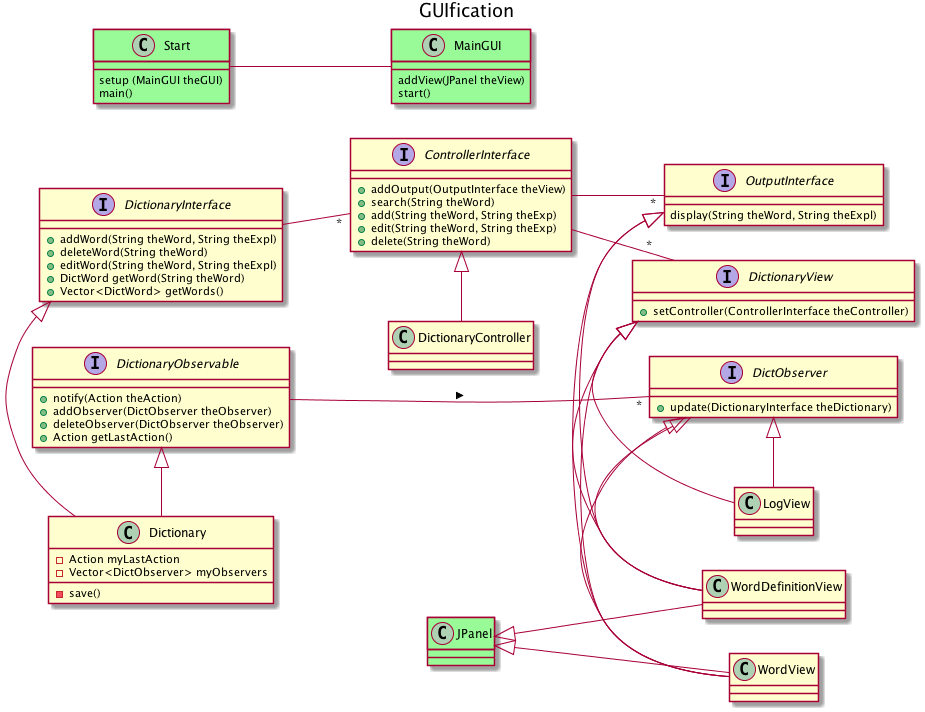
\includegraphics[width=.9\linewidth]{./FDictionaryClass4.png}
\end{document}